\section{Atmosphere/Interior model description}
% Delete the text and write your Theory/ Background Information here:
%------------------------------------
% \parencite[131,136]{Griffiths}. for citations
% \footnotetext{I used this word as an umbrella term for variables, constants, vectors, tensors and other things that can be measured/ found empirically.} for footnotes.
% \dpd[order]{}{} = display mode partial derivative
\subsection{Exo-REM}

As stated previously, Exo-REM \parencite{baudino_interpreting_2015} is a 1D radiative convective model with an out of equlibrium chemistry model \parencite{baudino_toward_2017} and a cloud model \parencite{charnay_self-consistent_2018}. For completeness we shall describe the basic workings of such a model. The more informed reader can skip this part.\par
If we consider a cylindrical element of atmosphere of surface $dS$ and length $dl$ then light moving through this element will gain and lose intensity following the following subsequent expressions. 

\begin{align} % Use & sign to align, use \nonumber \\ to write a line without number.
    dI_{\lambda -} = -\kappa_{\lambda} I_{\lambda_0} dS \nonumber \\
    dI_{\lambda +} = \epsilon_{\lambda} dS
\end{align}

With $I_{0}$ the initial intensity before entering the element, $\kappa$ the absorption coefficient and $\epsilon$ the emission coefficient. Combining these two expressions we get the radiative transfer equation.

\begin{align}
    \frac{dI_{\lambda}}{dS} = -\kappa_{\lambda} I_{\lambda} + \epsilon_{\lambda} \label{eq:pre-RTE}
\end{align}

\Cref{eq:pre-RTE} % Use \Cref at the start of a sentence and \cref mid sentence.
can be rewritten using the extinction coefficient $\tau$, which corresponds to the inverse of the average distance traveled by a photon before being scattered, whose expression is given by :

\begin{align}
    \tau_{\lambda} = \int \kappa_{\lambda} dS
\end{align}

As well as the source function given by :

\begin{align}
    S_{\lambda} = \frac{\epsilon_{\lambda}}{\kappa_{\lambda}}
\end{align}

Considering an atmosphere in local thermodynamic equilibrium defined as :

\begin{align}
    S_{\lambda} = B_{\lambda}
\end{align}

With B the idealized black body profile. we can hence write \cref{eq:pre-RTE} as :\par

\begin{align}
    \frac{dI_{\lambda}}{d\tau_{\lambda}} = -I_{\lambda} + B_{\lambda}
\end{align}

The absorption coefficient is in reality a sum of different contributions to the absorption of a parcel of atmosphere :

\begin{align}
    \kappa_{\lambda} = \kappa_{\lambda, chemistry} + \kappa_{\lambda, Rayleigh} + \nonumber \\
    \kappa_{\lambda, pair} + \kappa_{\lambda, aerosol}
\end{align}
With the various contributions defined as follows :\par
\begin{itemize}
    \item {$\kappa_{\lambda, chemistry}$} : Absorption by atoms/\\molecules.
    \item {$\kappa_{\lambda, Rayleigh}$} : Light scattered by \\fine particles.
    \item {$\kappa_{\lambda, pair}$} : Collision induced scattering.
    \item {$\kappa_{\lambda, aerosol}$ : Scattering, absorption due to\\ aerosols.}
\end{itemize}

While the specificity's of each of these coefficients is beyond the scope of the intended purpose of this work it is important to understand the expression of $\kappa_{\lambda, chemistry}$ to understand how Exo-REM links radiative transfer, chemistry and temperature profile. It's value is given by the following expression :

\begin{align}
    \kappa_{\lambda, chemistry} = \sum_{i=1}^{N_{species}} n_{i} \sigma_{\lambda,i}
\end{align}

With $N_{species}$ the molar concentration of species $i$ and $\sigma_{\lambda,i}$ the cross section which corresponds to the capacity to absorb at a given wavelength it is temperature and pressure dependant. Extensive experimental work is required to determine the values of cross sections. A humble physicist should keep in mind that the theoretical models used are only as good as the underlying experimental data and these values require updating regularly.\par

Resolving the radiative transfer equation at different levels (conversely optical depths) of the atmosphere does not suffice as we lack here the mechanical properties of layers of atmospheres at different thermodynamic conditions sat upon one another. Atmospheres on an averaged large scale can be quite accurately modeled using the hydrostatic balance equations linking mass $M$, pressure $P$, radius $r$, density $\rho$ using the universal gravitational constant $G$, which can be expressed as follows : \par

\begin{align}
    \frac{P}{dr} = -\frac{GM\rho(r)}{r^{2}} \label{eq:HBE}
\end{align}

The density $\rho$ here is linked to the temperature $T$, pressure $P$, mass $M$ using the ideal gas constant $R$, via the ideal gas law expressed as follows :

\begin{align}
    P = \frac{\rho R T}{M} \label{eq:IG}
\end{align}


The most attentive readers at this point might have alarm bells ringing as we mention deep atmosphere in the introduction where this law will hold up badly. This will be mentioned further in a subsequent section.\par

The fluxes considered in the radiative transfer equation are that of the stellar irradiation and the internal energy. They shall be subsequently expressed in temperatures using the Stefan Boltzmann approximation as shown in \cref{eq:SB}

\begin{align}
    \int_{0}^{\infty} \frac{\hbar}{4\pi^2c^2}\frac{\omega^3}{e^{\frac{\hbar\omega}{k_B T}}-1}\, d\omega = \sigma T^4 \label{eq:SB} \\
    \sigma = \frac{k_B^4}{4\pi^2c^2\hbar^3}\frac{\pi^4}{15} \nonumber
\end{align}

As such with the stated ingredients, it is possible to build a 1D atmosphere model like Exo-REM. Further physical aspects \parencite{charnay_self-consistent_2018} and the precise resolution method are beyond the current scope of this work but will be detailed in subsequent work. 

\subsection{Exoris}

As stated in the introduction, Exoris helps resolve the internal structure of a planet and relies on a library of equations of state. The range of parameters inputted into Exoris are give in \cref{tab:Exrs}.\par

\begin{table}[htb]%
\centering
\caption{Exoris parameters.}
	\label{tab:Exrs}
	\begin{tabular}{c}
		\toprule
		{$Exoris$}  \\
		\midrule
        \midrule
        {Mass of planet} \\
        \midrule
		{Mass fraction of core}   \\
        \midrule
		{Helium to hydrogen mass ratio}   \\
        \midrule
		{Water mass fraction}   \\
        \midrule
		{Proportion of rock in the core}   \\
        \midrule
        {Equation(s) of state for envelope}   \\
        \midrule
        {Equation(s) of state for core}   \\
        \midrule
        {Equation of state for ice}   \\
        \bottomrule
	\end{tabular}
\end{table}

Exoris seeks to solve the hydrostatic balance equation \cref{eq:HBE} using no longer the ideal gas law \cref{eq:IG} but rigorous equations of state (EOS) where the state of the considered matter varies depending on the pressure considered. To accomplish this, Exoris considers an adiabatic profile, where the entropy is defined by the helium to hydrogen mass fraction in the envelope at an initial "surface pressure".

\begin{align}
    S*n_{tot} = S_{h}*n_{h} + S_{he}*n_{he} + S_{mix}\label{eq:S1}
\end{align}

With $n_x$ the number of moles of each species and $S_{mix}$ the non linear mixing term. In practice we neglect $S_{mix}$ when estimating the adiabat. When using the mass fraction of helium $\gamma_{He}$, \cref{eq:S1} becomes :

\begin{align}
    S = S_{h}\frac{4-4\gamma_{He}}{4-3\gamma_{He}} + S_{he}\frac{\gamma_{He}}{4-3\gamma_{He}} \label{eq:S2}
\end{align}

It is also necessary to compute the "surface density" from the pressure and temperature conditions.

\begin{align}
    \frac{1}{\rho} = \frac{\alpha_H}{\rho_He} +  \frac{\alpha_{He}}{\rho_{He}} +  o(\delta V) \label{eq:D1}
\end{align}

Again here we will neglect mixing terms. Substituting the helium to hydrogen mass fraction ($\gamma_{He}$) into \cref{eq:D1} we get :

\begin{align}
    \rho = \frac{\rho_H*\rho_{He}}{\gamma_{He}*\rho_H + (1-\gamma_{He})*\rho_{He}} \label{eq:D2}
\end{align}

Once the planets entropy is fixed it is possible to determine the pressure temperature profile along a pressure grid by supposing that the system is adiabatic. Hence it is possible to derive a density profile and using \cref{eq:HBE} a radial profile. However it is necessary to take into account the different compositions within the planet and most notably the core. To do this, once an initial profile is constructed, the boundary for the core can be placed using the core mass fraction specified by the user. Doing so leads to Exoris reevaluating the temperature and density profile taking into account a new domain with a change of EOS, which will in turn lead to an adjustment of the boundary for the EOS change. Iterating this process a certain number of times leads to a converged profile which abides by the input parameters.\par

The EOS used by exoris for the hydrogen helium enveloppe is the S. Chabrier et al. 2019 updated dense hydrogen–helium mixtures EOS \parencite{chabrier_new_2019}. Benchmarks of the results produced with Exoris were done using the 1995 Saumon et al. SCVH equations \parencite{saumon_equation_1995}. \Cref{fig:M-R_benchmark},  where the underlying data is from Militzer et al. \parencite{militzer_ab_2013}, compares the two EOS, we chose to test various "surface pressures" in order to determine the impact that the inital entropy has on the outcome. We see that differences appear for high entropies (high temperature) and most notably at low mass. This diagram shows the intrinsic challenge of comparing models to one another which use different EOS. One has to be cautious. \par

\begin{figure}
    \centering
    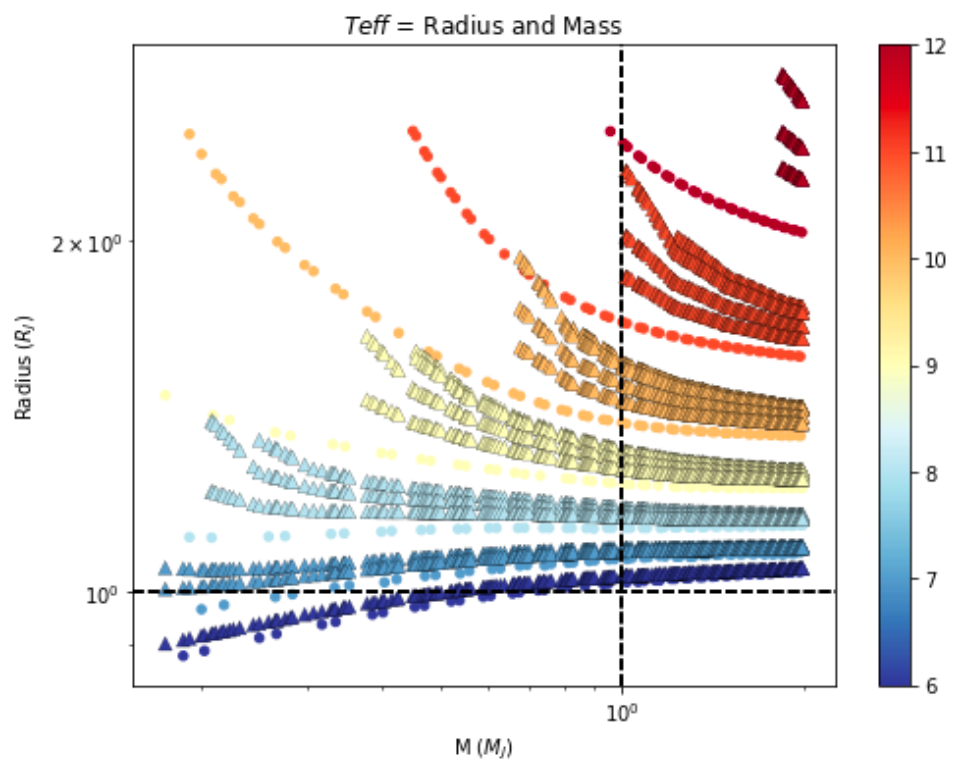
\includegraphics[width=0.48\textwidth]{Images/M-R_benchmark.png}
    \caption{Mass radius diagramme comparing Chabrier et al. 2019 (triangles) vs Saumon et al. 1995 circles with entropy on color axis in $K_b/el/mol$, multiple curves for different "surface pressures").}
    \label{fig:M-R_benchmark}
\end{figure}

Rigorous EOS are not plenteous and combining EOS is physically dubious as non linear terms that can have a strong impact are often neglected. In order to emulate higher atomic number compositions it is standard to increase the molecular concentration of other elements than hydrogen. In our case this would be H2O. We show how this is done in \cref{eq:compo} where $Z_m$ corresponds to higher atomic number elements.

\begin{align}
    \label{eq:compo}
    X_h + Y_{He} + Z_{H_2O} + Z_m = 1 \nonumber \\
    X_h + Y_{He} + Z'_{H_2O} = 1 \\ 
    with \,\,  Z'_{H_2O} = Z_{H_2O} + Z_m \nonumber 
\end{align}

By doing this, we need to change \cref{eq:S1} and \cref{eq:S2} to account for the added water in the envelope. We hence obtain the following equations :

\begin{align}
    S*n_{tot} = S_{H}n_{H} + S_{He}n_{He} + S_{He}n_{H_2O} + S_{mix}\label{eq:S3}
\end{align}

Again neglecting the ideal mixing term and using the helium to hydrogen mass fraction ($\gamma_{He}$) and water mass fraction ($\gamma_{H_2O}$), we obtain the following expression for $S$ :

\begin{align}
    x_{h} = \frac{36*(\gamma_{H_2O}-1)*(\gamma_{He}-1)}{\gamma_{H_2O}*(27*\gamma_{He}-34)-27*\gamma_{He}+36} \nonumber \\
    x_{he} = -\frac{9*(\gamma_{H_2O}-1)*\gamma_{He}}{\gamma_{H_2O}*(27*\gamma_{He}-34)-27*\gamma_{He}+36} \nonumber \\
    x_{h_2o} = \frac{2*\gamma_{H_2O}}{\gamma_{H_2O}*(27*\gamma_{He}-34)-27*\gamma_{He}+36} \nonumber \\
    S = S_{h}x_{H} + S_{he}x_{He} + S_{he}x_{H2O} \label{eq:S4}
\end{align}

Again we need to compute the "surface density" and the given pressure and temperature conditions. We hence add the density term for water onto \cref{eq:D1} and again neglecting mixing terms, we get :

\begin{align}
    \frac{1}{\rho} = \frac{\alpha_H}{\rho_He} +  \frac{\alpha_{He}}{\rho_{He}} +  \frac{\alpha_{H_2O}}{\rho_{H_2O}} \label{eq:D3}
\end{align}

Again here we will neglect mixing terms. Substituting he helium to hydrogen mass fraction ($\gamma_{He}$) and water mass fraction ($\gamma_{H_2O}$) into \cref{eq:D3} we get : 

\begin{align}
    \rho = \frac{rho_H*rho_{He}*rho_{H_2O}}{\begin{matrix}\rho_H*\rho_{He}*\gamma_{H_2O}\\-\rho_H*\rho_{H_2O}*(\gamma_{H_2O}-1)*\gamma_{He}\\+\rho_{He}*\rho_{H_2O}*(\gamma_{H_2O}-1)*(\gamma_{He}-1)\end{matrix}} \label{eq:D4}
\end{align}

Nullifying $\gamma_{H_2O}$ in \cref{eq:S4} and \cref{eq:D4} gives as expected \cref{eq:S2} and \cref{eq:D2}. Details on how \cref{eq:S4} and \cref{eq:D4} are derived are given in the annexes. Details on the derivation of $S_{mix}$ are equally given in the annexes.

Exoris is also capable of evaluating the gravitational moments but this is beyond the scope of this work.
